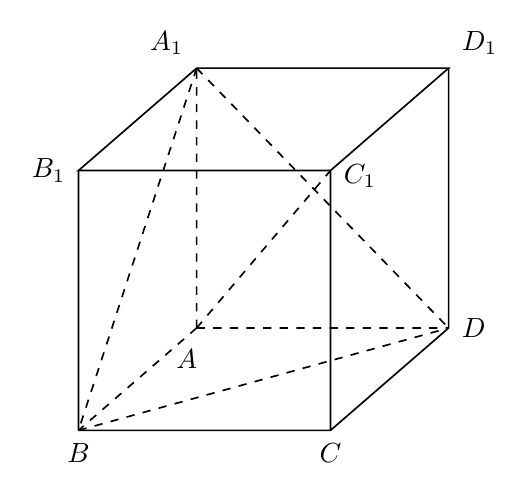
\begin{tikzpicture}[line width=0.6pt, font=\normalsize]
\tikzset{hid/.style={dashed}, lbl/.style={font=\normalsize, fill=white, inner sep=1.5pt}}
\coordinate (B) at (0,0); \coordinate (C) at (3.2,0); \coordinate (D) at (4.7,1.3); \coordinate (A) at (1.5,1.3);
\coordinate (B1) at (0,3.3); \coordinate (C1) at (3.2,3.3); \coordinate (D1) at (4.7,4.6); \coordinate (A1) at (1.5,4.6);
\draw (B)--(C)--(D) (B)--(B1) (C)--(C1) (D)--(D1);
\draw[hid] (A)--(B) (A)--(D) (A)--(A1);
\draw (B1)--(C1)--(D1)--(A1)--cycle;
\draw[hid] (A1)--(B) (A1)--(D) (B)--(D) (A)--(C1);
\node[lbl, below=3pt] at (B) {$B$};
\node[lbl, below=3pt] at (C) {$C$};
\node[lbl, right=3pt] at (D) {$D$};
\node[lbl, below left=2pt,fill=none,xshift=4.00bp,yshift=-4.00bp] at (A) {$A$};
\node[lbl, above left=3pt] at (A1) {$A_{1}$};
\node[lbl, left=3pt] at (B1) {$B_{1}$};
\node[lbl, right=3pt,fill=none,xshift=0.00bp,yshift=-2.00bp] at (C1) {$C_{1}$};
\node[lbl, above right=3pt] at (D1) {$D_{1}$};
\end{tikzpicture}
